% $Id: introduction.tex 34630 2013-04-29 22:53:51Z roldeman $

\section{Interpreting the results of SUSY searches at CMS}
\label{sec:susyModels}


% the susy production bit

The LHC is a 27km circumference hadron synchrotron built on the Franco-Swiss border \cite{LHCMachine} near Geneva. It ran from 2010 to 2013 colliding protons at centre-of-mass energies $\sqrt{s}=7$ and $8$ TeV (Run 1), with detectors built around the beam collecting up to $23.3$~fb$^{-1}$ of data. Preparations are currently underway for Run 2 of the LHC at a full operating energy of $\sqrt{s}=13$ to $14$ TeV in 2015. This upgrade will have a maximum instantaneous luminosity of $1.6\times10^{34}$~cm$^{-2}$s$^{-1}$, more than twice the peak of $7.7\times10^{33}$~cm$^{-2}$s$^{-1}$ reached in 2012 \cite{LHCLuminosityIPAC13}. With this increase in energy and luminosity, potential for the discovery of new physics at the energy frontier is high.  
\\\\
\subsection{Supersymmetry production at the LHC}
As the LHC is a hadron collider, the highest cross section SUSY production processes occur via the strong force \cite{SUSYprimerMartin:1997ns} \cite{SUSYxsections_NewAspectsof_pp_collisions}. These processes result in the production of squarks and gluinos, the SUSY particles with colour charge. In all favoured SUSY models, these relatively heavy particles decay within the detector to a weakly interacting LSP, usually a neutralino \cite{SUSYPhe_hadronic_states_Farrar:1978xj}. In collisions at the LHC this will appear as several hard jets with unbalanced momentum (missing energy). 
\\\\
To interpret the results of SUSY searches simplified models are used. These models include a smaller number of SUSY particles than the MSSM, but allow the representation of event topologies in a consistent way \cite{SimplifiedModelsAlves:2011wf} \cite{MathiasSUSYthesis}. A simplified model representation of hadronic SUSY production and decay can be seen in Fig.~\ref{fig:simpdecays}.
\begin{figure}
	\begin{center}
		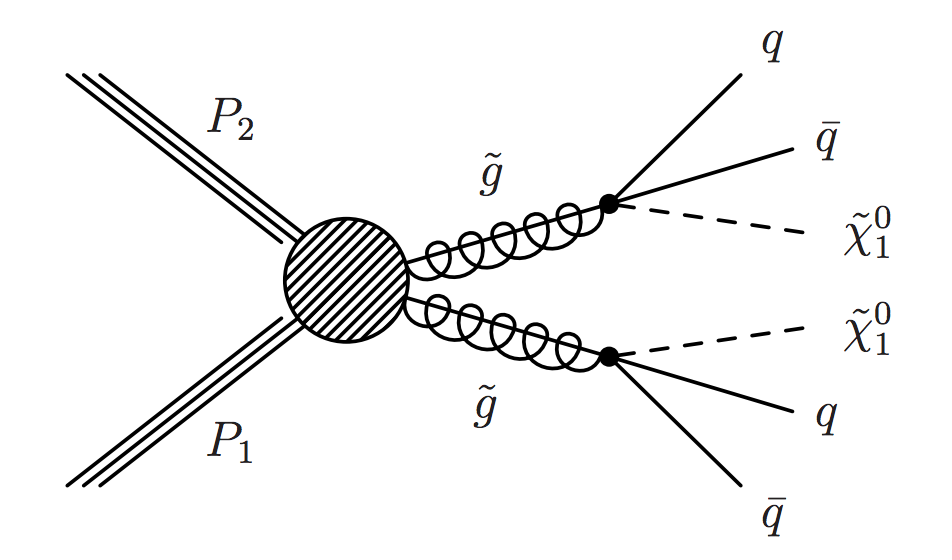
\includegraphics[width=0.4\linewidth]{T1simlifiedpp-gg-qqqqXX}\put(-32,133){(a)}
		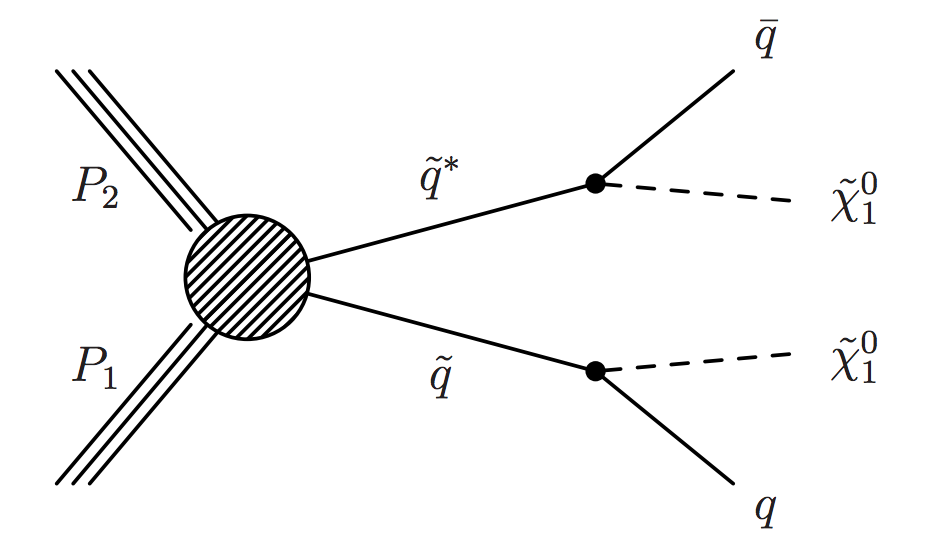
\includegraphics[width=0.4\linewidth]{T2simplifiedpp-qq-qqXX}\put(-32,133){(b)}
	\end{center}
	\caption{Simplified models of SUSY being produced at the LHC and decaying into hadrons plus missing energy \cite{MathiasSUSYthesis}}
	\label{fig:simpdecays}
\end{figure}
\\\\
The $7$ and $8$ TeV run of the LHC has not resulted in any observation of SUSY production as of yet. Instead, limits have been set on the mass of SUSY particles. It is possible that the mass of the SUSY particle has been outside of the energy range of the LHC. With the 2015 upgrade, the cross sections of such supersymmetric particles will increase by at least an order of magnitude, giving a large potential for discovery. It is also possible that the mass splitting of SUSY particles is small, known as compressed spectra. If this is the case the searches at the LHC are not as sensitive, as the energy of the jets produced in the decay to the LSP will be low. This results in a small visible component of missing energy. If SUSY exists at a scale that solves the hierarchy problem with minimal fine tuning, it should be seen at the LHC.




